% Options for packages loaded elsewhere
\PassOptionsToPackage{unicode}{hyperref}
\PassOptionsToPackage{hyphens}{url}
\documentclass[
  10pt,
]{article}
\usepackage{xcolor}
\usepackage[margin=2cm]{geometry}
\usepackage{amsmath,amssymb}
\setcounter{secnumdepth}{-\maxdimen} % remove section numbering
\usepackage{iftex}
\ifPDFTeX
  \usepackage[T1]{fontenc}
  \usepackage[utf8]{inputenc}
  \usepackage{textcomp} % provide euro and other symbols
\else % if luatex or xetex
  \usepackage{unicode-math} % this also loads fontspec
  \defaultfontfeatures{Scale=MatchLowercase}
  \defaultfontfeatures[\rmfamily]{Ligatures=TeX,Scale=1}
\fi
\usepackage{lmodern}
\ifPDFTeX\else
  % xetex/luatex font selection
\fi
% Use upquote if available, for straight quotes in verbatim environments
\IfFileExists{upquote.sty}{\usepackage{upquote}}{}
\IfFileExists{microtype.sty}{% use microtype if available
  \usepackage[]{microtype}
  \UseMicrotypeSet[protrusion]{basicmath} % disable protrusion for tt fonts
}{}
\makeatletter
\@ifundefined{KOMAClassName}{% if non-KOMA class
  \IfFileExists{parskip.sty}{%
    \usepackage{parskip}
  }{% else
    \setlength{\parindent}{0pt}
    \setlength{\parskip}{6pt plus 2pt minus 1pt}}
}{% if KOMA class
  \KOMAoptions{parskip=half}}
\makeatother
\usepackage{longtable,booktabs,array}
\usepackage{calc} % for calculating minipage widths
% Correct order of tables after \paragraph or \subparagraph
\usepackage{etoolbox}
\makeatletter
\patchcmd\longtable{\par}{\if@noskipsec\mbox{}\fi\par}{}{}
\makeatother
% Allow footnotes in longtable head/foot
\IfFileExists{footnotehyper.sty}{\usepackage{footnotehyper}}{\usepackage{footnote}}
\makesavenoteenv{longtable}
\setlength{\emergencystretch}{3em} % prevent overfull lines
\providecommand{\tightlist}{%
  \setlength{\itemsep}{0pt}\setlength{\parskip}{0pt}}
\usepackage[authoryear]{natbib}
\bibliographystyle{plainnat}
\usepackage{graphicx}
\renewcommand{\thefigure}{S\arabic{figure}}
\usepackage{bookmark}
\IfFileExists{xurl.sty}{\usepackage{xurl}}{} % add URL line breaks if available
\urlstyle{same}
\hypersetup{
  pdftitle={Supplementary Information to: Seed-dependent verdicts: a calibrated audit of attention-based binding-site explanations in drug--target interaction models},
  pdfauthor={Mahim Agarwal},
  hidelinks,
  pdfcreator={LaTeX via pandoc}}

\title{Supplementary Information to: Seed-dependent verdicts: a calibrated audit of attention-based binding-site explanations in drug--target interaction models}
\author{Mahim Agarwal}
\date{}

\begin{document}
\maketitle

\subsection{S1 Split sizes}\label{s1-split-sizes}

One fixed split per level; the rows below are the data rows of the split files, whose SHA-256 hashes are recorded in \texttt{data/splits/MANIFEST.json}. Only the random and cold-drug levels of KIBA were trained.

\textbf{Supplementary Table S1.} Rows per split (train / validation / test).

\begin{longtable}[]{@{}lllll@{}}
\toprule\noalign{}
dataset & level & train & validation & test \\
\midrule\noalign{}
\endhead
\bottomrule\noalign{}
\endlastfoot
DAVIS & random & 21,039 & 3,006 & 6,011 \\
DAVIS & cold-drug & 21,658 & 2,652 & 5,746 \\
DAVIS & cold-target & 21,080 & 2,992 & 5,984 \\
DAVIS & cold-pair & 15,190 & 264 & 1,144 \\
KIBA & random & 82,778 & 11,825 & 23,651 \\
KIBA & cold-drug & 83,807 & 12,073 & 22,374 \\
\end{longtable}

Cold-pair discards every pair with exactly one unseen entity, so it trains on fewer rows than the random level (15,190 against 21,039 on DAVIS). A volume-matched control for this exists for XAttn-Ref but is not used in this manuscript.

\subsection{S2 Training recipes}\label{s2-training-recipes}

Each published model is trained from its vendored repository (\texttt{baselines/}) with its authors' optimiser, learning rate, batch size and tokeniser; only data loading is replaced. The commands are built by \texttt{src/cloud/recipes.py}, which reproduces the flags of the notebooks that trained the cells.

\textbf{Supplementary Table S2.} Optimiser, learning rate and batch size per model.

\begin{longtable}[]{@{}
  >{\raggedright\arraybackslash}p{(\linewidth - 8\tabcolsep) * \real{0.2000}}
  >{\raggedright\arraybackslash}p{(\linewidth - 8\tabcolsep) * \real{0.2000}}
  >{\raggedright\arraybackslash}p{(\linewidth - 8\tabcolsep) * \real{0.2000}}
  >{\raggedright\arraybackslash}p{(\linewidth - 8\tabcolsep) * \real{0.2000}}
  >{\raggedright\arraybackslash}p{(\linewidth - 8\tabcolsep) * \real{0.2000}}@{}}
\toprule\noalign{}
\begin{minipage}[b]{\linewidth}\raggedright
model
\end{minipage} & \begin{minipage}[b]{\linewidth}\raggedright
optimiser
\end{minipage} & \begin{minipage}[b]{\linewidth}\raggedright
learning rate
\end{minipage} & \begin{minipage}[b]{\linewidth}\raggedright
batch
\end{minipage} & \begin{minipage}[b]{\linewidth}\raggedright
notes
\end{minipage} \\
\midrule\noalign{}
\endhead
\bottomrule\noalign{}
\endlastfoot
DeepDTA & Adam & 0.001 & 256 & PyTorch port; patience 10 \\
HyperAttentionDTI & AdamW, cyclic learning rate & 0.00005 & 32 & weight decay 0.0001 on weights, none on biases \\
MolTrans & Adam & 0.0001 & 16 & configuration \texttt{BIN\_config\_DBPE} \\
DrugBAN & Adam & 0.00005 & 64 & domain adaptation off; DAVIS only \\
XAttn-Ref & Adam, reduce-on-plateau & 0.001 & 64 & learning rate halved after 5 epochs without improvement \\
\end{longtable}

\textbf{Mixed precision on KIBA.} DeepDTA and HyperAttentionDTI were trained with mixed precision (float16 autocast) on KIBA, as recorded in each cell's results file; MolTrans (whose layer normalisation underflows in half precision) and XAttn-Ref were trained in full precision, as was every DAVIS cell. The choice was validated beforehand on one DAVIS cell, HyperAttentionDTI at cold-pair, with three seeds per arm: test AUROC was 0.694 $\pm$ 0.038 in full precision (Kaggle, torch 2.10) and 0.681 $\pm$ 0.068 in mixed precision (Colab, torch 2.11), and precision@10 was 0.022 $\pm$ 0.012 against 0.023 $\pm$ 0.018, so the mixed-precision means lay within the full-precision seed spread. Three seeds per arm detect only a gross effect and cannot show equivalence, and the two arms also differed in library version and machine.

Two defects in the vendored MolTrans code are contained without editing it. Its forward pass reshapes by the configured batch size, so a final partial batch would be scored wrongly; the batch size is set per batch (\texttt{\_fit\_batch\_size}). And one functional dropout call omits the training flag (\texttt{baselines/MolTrans/models.py:103}), so dropout stays active at inference: its test metrics are one draw of that noise, as in the published model. On DAVIS cold-pair, six further draws of one checkpoint spread its test AUROC over 0.5862--0.5954, and the recorded value lies inside that range.

\textbf{Supplementary Table S3.} Test AUROC, mean $\pm$ standard deviation over three training seeds. ``Sequence-unseen'' scores only test targets whose sequence does not occur in training (Section 3.6). DrugBAN has no KIBA cells. \emph{Source:} \texttt{results/accuracy\_v2/by\_model.csv}.

\begin{longtable}[]{@{}
  >{\raggedright\arraybackslash}p{(\linewidth - 16\tabcolsep) * \real{0.1111}}
  >{\raggedright\arraybackslash}p{(\linewidth - 16\tabcolsep) * \real{0.1111}}
  >{\raggedright\arraybackslash}p{(\linewidth - 16\tabcolsep) * \real{0.1111}}
  >{\raggedright\arraybackslash}p{(\linewidth - 16\tabcolsep) * \real{0.1111}}
  >{\raggedright\arraybackslash}p{(\linewidth - 16\tabcolsep) * \real{0.1111}}
  >{\raggedright\arraybackslash}p{(\linewidth - 16\tabcolsep) * \real{0.1111}}
  >{\raggedright\arraybackslash}p{(\linewidth - 16\tabcolsep) * \real{0.1111}}
  >{\raggedright\arraybackslash}p{(\linewidth - 16\tabcolsep) * \real{0.1111}}
  >{\raggedright\arraybackslash}p{(\linewidth - 16\tabcolsep) * \real{0.1111}}@{}}
\toprule\noalign{}
\begin{minipage}[b]{\linewidth}\raggedright
model
\end{minipage} & \begin{minipage}[b]{\linewidth}\raggedright
DAVIS random
\end{minipage} & \begin{minipage}[b]{\linewidth}\raggedright
DAVIS cold-drug
\end{minipage} & \begin{minipage}[b]{\linewidth}\raggedright
DAVIS cold-target
\end{minipage} & \begin{minipage}[b]{\linewidth}\raggedright
cold-target, sequence-unseen
\end{minipage} & \begin{minipage}[b]{\linewidth}\raggedright
DAVIS cold-pair
\end{minipage} & \begin{minipage}[b]{\linewidth}\raggedright
cold-pair, sequence-unseen
\end{minipage} & \begin{minipage}[b]{\linewidth}\raggedright
KIBA random
\end{minipage} & \begin{minipage}[b]{\linewidth}\raggedright
KIBA cold-drug
\end{minipage} \\
\midrule\noalign{}
\endhead
\bottomrule\noalign{}
\endlastfoot
MolTrans & 0.923 $\pm$ 0.002 & 0.685 $\pm$ 0.019 & 0.874 $\pm$ 0.006 & 0.833 $\pm$ 0.008 & 0.568 $\pm$ 0.025 & 0.532 $\pm$ 0.029 & 0.919 $\pm$ 0.004 & 0.812 $\pm$ 0.009 \\
HyperAttentionDTI & 0.937 $\pm$ 0.005 & 0.760 $\pm$ 0.042 & 0.915 $\pm$ 0.001 & 0.893 $\pm$ 0.001 & 0.694 $\pm$ 0.038 & 0.713 $\pm$ 0.050 & 0.933 $\pm$ 0.001 & 0.844 $\pm$ 0.004 \\
DrugBAN & 0.891 $\pm$ 0.006 & 0.695 $\pm$ 0.033 & 0.846 $\pm$ 0.010 & 0.801 $\pm$ 0.012 & 0.620 $\pm$ 0.031 & 0.559 $\pm$ 0.040 & --- & --- \\
XAttn-Ref & 0.924 $\pm$ 0.001 & 0.721 $\pm$ 0.008 & 0.857 $\pm$ 0.011 & 0.835 $\pm$ 0.015 & 0.624 $\pm$ 0.099 & 0.607 $\pm$ 0.128 & 0.894 $\pm$ 0.011 & 0.807 $\pm$ 0.009 \\
DeepDTA & 0.929 $\pm$ 0.002 & 0.692 $\pm$ 0.044 & 0.907 $\pm$ 0.003 & 0.884 $\pm$ 0.003 & 0.728 $\pm$ 0.035 & 0.749 $\pm$ 0.044 & 0.918 $\pm$ 0.001 & 0.832 $\pm$ 0.001 \\
\end{longtable}

\subsection{S4 Readout sensitivity}\label{s4-readout-sensitivity}

A multi-head, multi-channel attention model must be reduced to one weight per residue. Besides the primary readout (Section 2.2), the following reductions were scored with the same pipeline: XAttn-Ref's protein self-attention, HyperAttentionDTI's maximum over channels and its receptive-field spread, MolTrans's maximum over heads and its first layer, MolTrans's drug $\times$ protein interaction map, and DrugBAN's maximum over atoms and receptive-field spread. The reductions disagree most for HyperAttentionDTI against the KLIFS pocket at the cold-target level:

\textbf{Supplementary Table S4.} HyperAttentionDTI, KLIFS pocket, DAVIS cold-target.

\begin{longtable}[]{@{}lll@{}}
\toprule\noalign{}
readout & precision@10 (mean $\pm$ SD over seeds) & chance \\
\midrule\noalign{}
\endhead
\bottomrule\noalign{}
\endlastfoot
primary (channel mean) & 0.186 $\pm$ 0.032 & 0.140 \\
maximum over channels & 0.367 $\pm$ 0.104 & 0.140 \\
receptive-field spread & 0.081 $\pm$ 0.046 & 0.140 \\
\end{longtable}

The readout-comparison table is written by the readout runs to the checkpoint-side results folder and is versioned in the repository as \texttt{results/readout\_comparison.csv} (a byte-identical copy). Drug dependence of each readout was measured on 25 proteins with four drugs each: the top ten residues are identical across drugs in 100\% of drug pairs for MolTrans's primary readout, in 72\% for HyperAttentionDTI's and in 0\% for DrugBAN's. MolTrans's drug $\times$ protein interaction map, scored as a readout variant, gives identical top-ten residues across drugs in 0\% of the same 150 drug pairs.

\subsection{S5 Integrated gradients on the same weights (confirmatory)}\label{s5-integrated-gradients-on-the-same-weights-confirmatory}

Integrated gradients \citep{Sundararajan2017} (32 steps) on the same checkpoints localise better than the attention in some cells, not all. For XAttn-Ref at DAVIS cold-drug, IG reaches 3.16 {[}2.40, 4.40{]}$\times$ chance in the pocket against the attention's 2.10 {[}1.83, 2.36{]}$\times$. For HyperAttentionDTI at KIBA cold-drug, IG's point estimate against UniProt residues, 1.90$\times$, is above the attention's 0.94 {[}0.71, 1.19{]}$\times$, but with seeds resampled its interval, {[}0.63, 3.39{]}, includes parity. IG coverage is partial (this Supplement, S6), and we read it only as evidence that a weak attention map can under-report what a model represents.

\subsection{S6 Where each instrument was run}\label{s6-where-each-instrument-was-run}

\begin{longtable}[]{@{}
  >{\raggedright\arraybackslash}p{(\linewidth - 4\tabcolsep) * \real{0.3333}}
  >{\raggedright\arraybackslash}p{(\linewidth - 4\tabcolsep) * \real{0.3333}}
  >{\raggedright\arraybackslash}p{(\linewidth - 4\tabcolsep) * \real{0.3333}}@{}}
\toprule\noalign{}
\begin{minipage}[b]{\linewidth}\raggedright
instrument
\end{minipage} & \begin{minipage}[b]{\linewidth}\raggedright
code
\end{minipage} & \begin{minipage}[b]{\linewidth}\raggedright
outputs
\end{minipage} \\
\midrule\noalign{}
\endhead
\bottomrule\noalign{}
\endlastfoot
audit with Holm (primary record) & \texttt{src/evaluation/run\_audit.py} & \texttt{results/analysis\_\{davis,kiba\}\_policyA/audit\_*\_10k\_permutations.*} \\
UniProt and KLIFS ladders & \texttt{src/evaluation/run\_ladder.py} & \texttt{results/analysis\_*\_policyA*/} \\
enrichment and faithfulness intervals (two-way: seeds and targets resampled; quoted in the text) & \texttt{src/evaluation/effects\_v2.py\ -\/-resample\ seeds\_and\_targets} & \texttt{results/effects\_v2\_2d/} \\
enrichment and faithfulness intervals (targets only, as the amendment specified; comparison) & \texttt{src/evaluation/effects\_v2.py} & \texttt{results/effects\_v2/} \\
readout comparison & readout runs (checkpoint-side), copied byte-identical & \texttt{results/readout\_comparison.csv} \\
seed agreement & \texttt{src/evaluation/seed\_agreement.py} & \texttt{results/seed\_agreement.md} \\
positive control & \texttt{src/evaluation/positive\_control.py} & \texttt{results/positive\_control\_\{davis,kiba\}.md} \\
positional and residue nulls & \texttt{src/evaluation/positional\_control.py} & all four attention models on DAVIS, UniProt and KLIFS (\texttt{results/analysis\_davis\_policyA/positional\_control\_*}); HyperAttentionDTI and MolTrans on KIBA against both ground truths, XAttn-Ref on KIBA against KLIFS only (\texttt{results/analysis\_kiba\_policyA/positional\_control\_*}) \\
faithfulness (committed means) & \texttt{src/evaluation/run\_faithfulness.py}, \texttt{token\_faithfulness.py} & \texttt{results/analysis\_*\_policyA/} \\
accuracy and accuracy-vs-localization & \texttt{src/evaluation/accuracy\_table.py} & \texttt{results/accuracy\_v2/} \\
leakage retraining & \texttt{src/evaluation/leakage\_retrain.py} & \texttt{results/leakage\_retrain\_davis.md} \\
\end{longtable}

\subsection{S7 Threats to validity: the problem log}\label{s7-threats-to-validity-the-problem-log}

\textbf{Supplementary Table S5.} Problems found during the project, their effect, and how each is handled. ``Open'' marks a problem that remains a limitation of this manuscript.

\begin{longtable}[]{@{}
  >{\raggedright\arraybackslash}p{(\linewidth - 8\tabcolsep) * \real{0.2000}}
  >{\raggedright\arraybackslash}p{(\linewidth - 8\tabcolsep) * \real{0.2000}}
  >{\raggedright\arraybackslash}p{(\linewidth - 8\tabcolsep) * \real{0.2000}}
  >{\raggedright\arraybackslash}p{(\linewidth - 8\tabcolsep) * \real{0.2000}}
  >{\raggedright\arraybackslash}p{(\linewidth - 8\tabcolsep) * \real{0.2000}}@{}}
\toprule\noalign{}
\begin{minipage}[b]{\linewidth}\raggedright
\#
\end{minipage} & \begin{minipage}[b]{\linewidth}\raggedright
problem
\end{minipage} & \begin{minipage}[b]{\linewidth}\raggedright
effect if unhandled
\end{minipage} & \begin{minipage}[b]{\linewidth}\raggedright
handling
\end{minipage} & \begin{minipage}[b]{\linewidth}\raggedright
status / evidence
\end{minipage} \\
\midrule\noalign{}
\endhead
\bottomrule\noalign{}
\endlastfoot
a & DAVIS mutants carry the wild-type sequence & ``unseen'' targets partly seen; cold accuracy inflated & sequence policy; leak quantified by retraining & handled --- \texttt{results/sequence\_audit\_davis.md}, \texttt{results/leakage\_retrain\_davis.md} \\
b & vendored MolTrans re-seeds the random generator on import & every seed trains as the first seed & seed after import; import wrapped to preserve generator state; affected cells retrained & handled --- \texttt{tests/test\_train\_moltrans.py}, \texttt{tests/test\_integrity\_rng\_seeds.py} \\
c & masking arms not size-matched for a sub-word model & random arm is roughly twice the intervention, biasing faithfulness & token-matched control & handled --- \texttt{results/mask\_comparability\_davis.md} \\
d & match quality of MolTrans's token-matched control not recorded; matching can fail when attention sits at a sequence end & some control draws may exceed the tolerance & reported as a limitation & open --- ledger T02, discovered items \\
e & the primary readouts may differ from the maps the papers display; not confirmed against their figures & a primary verdict may concern a different map & alternative readouts scored as variants (MolTrans's interaction map; others in S4) & open --- \texttt{docs/readout\_sources.md} \\
f & permutation resolution was 500 in the original audit & smallest p close to the smallest Holm threshold & 10,000-permutation audit is the primary record; verdicts unchanged & handled --- \texttt{docs/PROTOCOL\_AMENDMENT\_v2.md} §2.1 \\
g & two vendored repositories ship a module with the same name & one model silently loads the other's code & modules loaded in isolation & handled --- \texttt{tests/test\_drugban\_import\_isolation.py} \\
h & the analysis runner skipped finished outputs & a partial grid would freeze missing levels silently & runner refuses a changed grid outside a scratch folder & handled --- \texttt{src/evaluation/run\_all.py}, \texttt{tests/test\_integrity\_grid.py} \\
i & faithfulness depends on the number of residues masked & a verdict could reflect the chosen k & k = 10 fixed in advance; k = 50 as sensitivity for two models & handled --- \texttt{results/faithfulness\_k50\_davis/} \\
j & DrugBAN's loader caps molecules at a fixed atom count & rows silently dropped & collector skips and fails loudly above a limit; the limit is a floor of three rows or 1\%, whichever is larger & handled; limit wording corrected --- ledger D6 \\
k & MolTrans keeps dropout on at inference & single-draw test metrics and faithfulness re-runs differ slightly & forward passes seeded for explanations; stated & open (as published) --- ledger T04, T05 \\
l & HyperAttentionDTI masking would have written alanine; its positive logit was read alone & a different intervention and a quantity that can move without the prediction & mask to \texttt{X} via each model's tokeniser; log-odds & handled --- \texttt{src/evaluation/residue\_space.py} \\
m & ground-truth residues numbered along UniProt, not along the dataset sequence & sites point at the wrong residue or past the end & alignment-based re-numbering; the positive control fails on un-renumbered sites & handled --- \texttt{src/data/align\_ground\_truth.py} \\
n & tied attention broken by a stable sort & positional artefact read as quality & ties broken at random & handled --- \texttt{src/evaluation/precision\_at\_k.py} \\
o & Holm families enlarged after first results & post-hoc family definition & disclosed; frozen by dated amendment & disclosed --- \texttt{docs/PROTOCOL\_AMENDMENT\_v2.md} G4 \\
p & faithfulness re-runs do not reproduce the committed means exactly for MolTrans and for HyperAttentionDTI on DAVIS & intervals describe a re-run draw & committed means stay primary; verdict signs unchanged & open --- ledger T05 \\
q & an interrupted checkpoint was once analysed & a partly trained model scored as final & runner refuses a checkpoint without its results file & handled --- \texttt{CLAUDE.md} §6 \\
r & no random-generator state or initial-weight hash recorded for the trained cells & seed distinctness not provable after the fact & recorded for all future cells by the cloud harness & open for existing cells --- ledger T01 \\
s & DAVIS cold-pair validation contains seen-by-sequence targets & checkpoint selection influenced by the leak & cannot be undone without retraining & open --- \texttt{results/sequence\_audit\_davis.md} \\
t & no conservation control for the pocket enrichment & enrichment may reflect conserved residues & none & open --- amendment A1/A7 \\
u & the sampled 1,000-permutation per-seed p put one seed on the $\alpha$ line & headline disagreement count 12 vs 11 & exact p recomputed independently; 11 reported, 12 disclosed & handled --- \texttt{scripts/certification/step1b\_exact\_p\_validation.py} \\
v & the leak's all-rows AUROC effect is not distinguishable from zero with three seeds & a small, insignificant number quoted as a finding & not quoted; leaked-row effect reported with its test & handled --- \texttt{results/certification/step3\_leak.txt} \\
w & the same seed and the same initial weights give different results on re-running (one pair of runs) & part of the ``seed'' variation is run-to-run variation, and the cause of the map disagreement is not isolated & stated as a limitation; both canary runs are reported & open --- \texttt{docs/canary\_attempts/README.md} \\
x & the 10,000-permutation audit's cell p-values differ from an exact recomputation by up to 0.0511 on DAVIS and by 0.54 in one KIBA cell; the cause is not established & the survivor counts could differ & Holm recomputed from the exact p-values leaves the same survivors & open --- \texttt{results/certification/step4\_holm.txt} \\
\end{longtable}

For (c), 47.9\% of tokens change under the attended arm and 95.0\% under an unmatched random arm, on 20 DAVIS proteins.

\subsection{S8 Supplementary figures}\label{s8-supplementary-figures}

\begin{figure}[t]
\centering
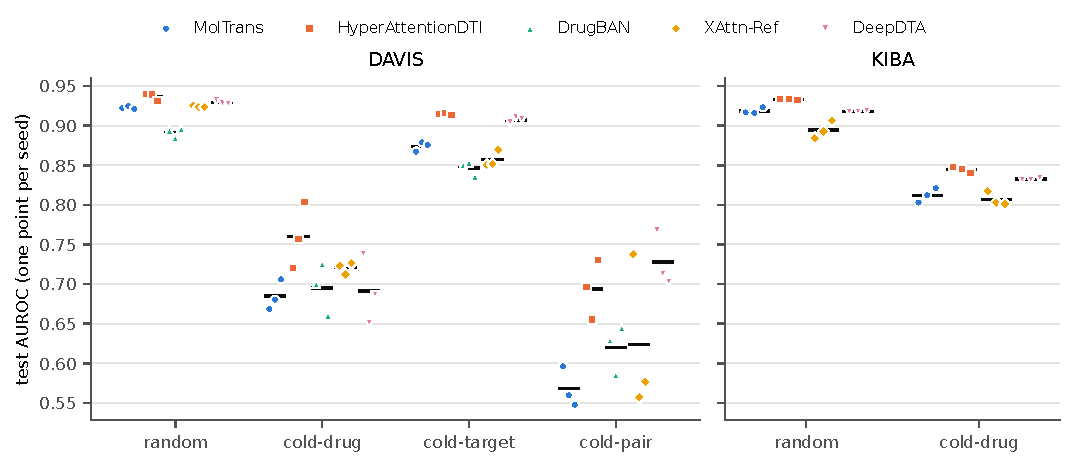
\includegraphics[width=\linewidth]{figures/fig3_accuracy.pdf}
\caption{\textbf{Predictive accuracy per training seed.} Test AUROC of every cell (points, one per seed; bar = mean) on the uncorrected test sets. DeepDTA has no attention and anchors accuracy. KIBA has two levels (random, cold-drug) and no DrugBAN cells.}
\label{fig:supplementaryfigures1}
\end{figure}

\begin{figure}[t]
\centering
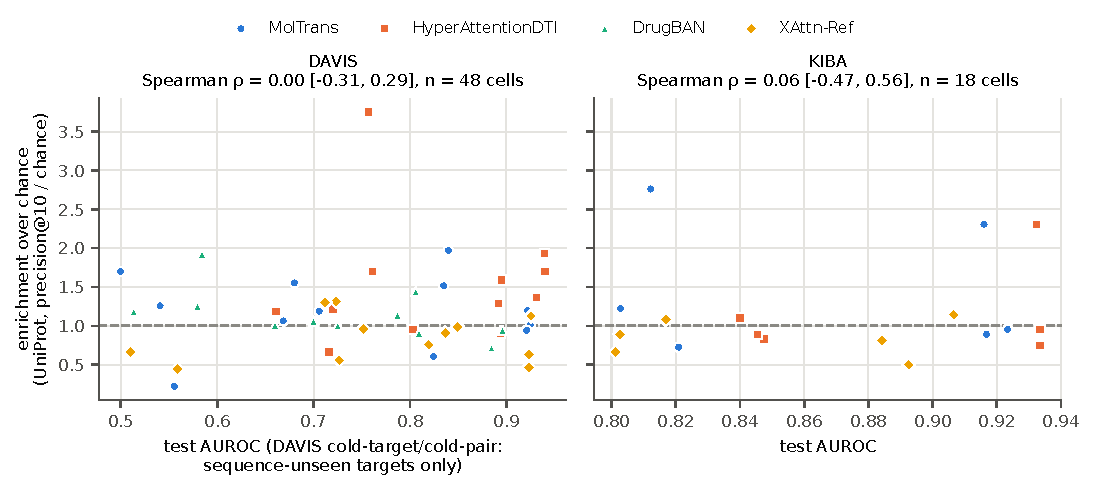
\includegraphics[width=\linewidth]{figures/fig4_accuracy_vs_localization.pdf}
\caption{\textbf{Accuracy does not predict localisation.} One point per attention-model cell and seed: test AUROC against enrichment over chance (UniProt, precision@10 divided by chance). For DAVIS cold-target and cold-pair, AUROC is scored on sequence-unseen targets, the same policy the explanation metrics use. Panel titles give Spearman's $\rho$ with a 95\% bootstrap interval over cells.}
\label{fig:supplementaryfigures2}
\end{figure}

\bibliography{references}

\end{document}
